\documentclass[11pt]{article}

% Change "review" to "final" to generate the final (sometimes called camera-ready) version.
% Change to "preprint" to generate a non-anonymous version with page numbers.
\usepackage[review]{acl}

% Standard package includes
\usepackage{times}
\usepackage{latexsym}

% For proper rendering and hyphenation of words containing Latin characters (including in bib files)
\usepackage[T1]{fontenc}
% For Vietnamese characters
% \usepackage[T5]{fontenc}
% See https://www.latex-project.org/help/documentation/encguide.pdf for other character sets

% This assumes your files are encoded as UTF8
\usepackage[utf8]{inputenc}

% This is not strictly necessary, and may be commented out,
% but it will improve the layout of the manuscript,
% and will typically save some space.
\usepackage{microtype}

% This is also not strictly necessary, and may be commented out.
% However, it will improve the aesthetics of text in
% the typewriter font.
\usepackage{inconsolata}

%Including images in your LaTeX document requires adding
%additional package(s)
\usepackage{graphicx}

\usepackage{amsmath} 

% If the title and author information does not fit in the area allocated, uncomment the following
%
%\setlength\titlebox{<dim>}
%
% and set <dim> to something 5cm or larger.

\newcommand{\passone}{\texttt{pass\^{}1}}
\newcommand{\passk}{\texttt{pass\^{}k}}
\newcommand{\asr}{\text{ASR}}

% Author information can be set in various styles:
% For several authors from the same institution:
% \author{Author 1 \and ... \and Author n \\
%         Address line \\ ... \\ Address line}
% if the names do not fit well on one line use
%         Author 1 \\ {\bf Author 2} \\ ... \\ {\bf Author n} \\
% For authors from different institutions:
% \author{Author 1 \\ Address line \\  ... \\ Address line
%         \And  ... \And
%         Author n \\ Address line \\ ... \\ Address line}
% To start a separate ``row'' of authors use \AND, as in
% \author{Author 1 \\ Address line \\  ... \\ Address line
%         \AND
%         Author 2 \\ Address line \\ ... \\ Address line \And
%         Author 3 \\ Address line \\ ... \\ Address line}

\author{First Author \\
  Affiliation / Address line 1 \\
  Affiliation / Address line 2 \\
  Affiliation / Address line 3 \\
  \texttt{email@domain} \\\And
  Second Author \\
  Affiliation / Address line 1 \\
  Affiliation / Address line 2 \\
  Affiliation / Address line 3 \\
  \texttt{email@domain} \\}

%\author{
%  \textbf{First Author\textsuperscript{1}},
%  \textbf{Second Author\textsuperscript{1,2}},
%  \textbf{Third T. Author\textsuperscript{1}},
%  \textbf{Fourth Author\textsuperscript{1}},
%\\
%  \textbf{Fifth Author\textsuperscript{1,2}},
%  \textbf{Sixth Author\textsuperscript{1}},
%  \textbf{Seventh Author\textsuperscript{1}},
%  \textbf{Eighth Author \textsuperscript{1,2,3,4}},
%\\
%  \textbf{Ninth Author\textsuperscript{1}},
%  \textbf{Tenth Author\textsuperscript{1}},
%  \textbf{Eleventh E. Author\textsuperscript{1,2,3,4,5}},
%  \textbf{Twelfth Author\textsuperscript{1}},
%\\
%  \textbf{Thirteenth Author\textsuperscript{3}},
%  \textbf{Fourteenth F. Author\textsuperscript{2,4}},
%  \textbf{Fifteenth Author\textsuperscript{1}},
%  \textbf{Sixteenth Author\textsuperscript{1}},
%\\
%  \textbf{Seventeenth S. Author\textsuperscript{4,5}},
%  \textbf{Eighteenth Author\textsuperscript{3,4}},
%  \textbf{Nineteenth N. Author\textsuperscript{2,5}},
%  \textbf{Twentieth Author\textsuperscript{1}}
%\\
%\\
%  \textsuperscript{1}Affiliation 1,
%  \textsuperscript{2}Affiliation 2,
%  \textsuperscript{3}Affiliation 3,
%  \textsuperscript{4}Affiliation 4,
%  \textsuperscript{5}Affiliation 5
%\\
%  \small{
%    \textbf{Correspondence:} \href{mailto:email@domain}{email@domain}
%  }
%}

\title{DUMA-Bench: A Dual-Control Multi-Agent Benchmark for Evaluating LLM Agent Security}

\begin{document}

\maketitle

\begin{abstract}

LLM-based agents increasingly operate in environments where they interact with users, tools, and external systems. Yet most security evaluations assume passive users and static control, ignoring the interactive dynamics that shape real agent behavior. We introduce \textbf{DUMA-Bench}, a benchmark and evaluation protocol for measuring agent security under \emph{dual-control} interaction, where both the agent and the user can influence the shared environment state. DUMA-Bench extends $\tau^2$-bench with adversarial environments covering eight vulnerability classes, including RAG poisoning, cross-agent manipulation, and unsafe output handling. We evaluate \textbf{14 models from five model families} (OpenAI, Anthropic, DeepSeek, Qwen, and Z.ai) across eight domains and multiple user-behavior regimes. Across our experiments, introducing dual-control interaction increases the attack success rate from \textbf{25\%} to \textbf{40\%}. These results show that agent security is not solely a property of the model but emerges from the interaction between the model, the user, and the environment. DUMA-Bench provides a missing evaluation layer for studying security in realistic agent deployments.

\end{abstract}


\section{Introduction}

Large language models (LLMs) are increasingly deployed as autonomous or semi-autonomous agents that interact with external tools, environments, and users. 
In such systems, security vulnerabilities often emerge not from a single model response but from the interaction dynamics between the model, the user, and the environment.
Most existing safety benchmarks evaluate LLMs under a \emph{passive-user} assumption, where the model receives a fixed prompt and produces a single response. 
However, real-world agent systems involve iterative interaction, tool use, and environment updates. 
These additional interaction channels create new opportunities for adversarial manipulation that are not captured by traditional prompt-based evaluation.
In this work, we introduce \textbf{DUMA-Bench}, a benchmark designed to evaluate LLM security under \emph{dual-control interaction}, where both the user and the model can influence the environment across multiple steps. 
This setting captures realistic agent workflows such as email handling, collaborative document editing, retrieval systems, and customer support tools.
Our key hypothesis is that security vulnerabilities depend not only on the model itself but also on the \emph{interaction regime}. 
We therefore compare two evaluation settings: a traditional passive-user setup and a dual-control interaction setup that allows iterative environment manipulation.
Across 14 models from five model families, we find that security performance can degrade substantially when moving from passive to interactive settings. 
In particular, attack success rates increase across most domains when adversarial interaction is allowed, suggesting that traditional prompt-based benchmarks systematically underestimate risk in agent systems.

Our contributions are:
\begin{itemize}
\item We introduce \textbf{DUMA-Bench}, a benchmark for evaluating LLM security under interactive dual-control settings.
\item We propose a unified evaluation protocol using Attack Success Rate (ASR) as the primary metric and pass@k to capture stochastic interaction trajectories.
\item We evaluate 14 models across multiple domains and show that interactive environments significantly increase vulnerability compared to passive evaluation.
\end{itemize}

\textbf{YES?? : Code, benchmark tasks, and evaluation scripts will be released to facilitate reproducible research on interactive agent security.}

\section{Related Work}

\paragraph{Agent interaction and coordination benchmarks.}

Early evaluation of LLM-based agents focused on single-agent reasoning and tool use under centralized control. Benchmarks such as AgentBench~\cite{liu2023agentbench} evaluated instruction following and task completion but did not model interaction with dynamic users or collaborators. More recent work studies coordination in shared environments. The $\tau$-bench framework~\cite{yao2024tau} introduced environments where agents interact with users whose actions can modify the environment state. $\tau^2$-bench~\cite{barres2025tau} formalized this interaction as a two-party Dec-POMDP~\cite{amato2013decentralized} and showed that shared control alone can significantly affect agent performance. However, these coordination benchmarks do not model adversarial behavior or security threats.

\paragraph{Security evaluation of LLM agents.}

A separate line of work studies the security of LLM-based agents. Agent Security Bench~\cite{zhang2025agent} introduces structured attacks such as prompt injection and tool misuse. Agent Dojo~\cite{debenedetti2024agentdojo} evaluates agent robustness in dynamic environments with corrupted tool outputs and malicious instructions. Other work studies specific attack surfaces such as prompt injection, tool manipulation, and data leakage. While these benchmarks provide valuable insights into agent vulnerabilities, they typically assume passive users and evaluate attacks in single-controller settings.

\paragraph{Environment-level and RAG attacks.}

The integration of retrieval and external data sources into agent systems introduces additional attack surfaces. Prior work demonstrates that poisoning retrieved documents or knowledge bases can significantly increase attack success rates~\cite{zou2025poisonedrag}. Related work studies agent-specific backdoors~\cite{chen2024agentpoison} and environment-triggered attacks~\cite{wang2024badagent}. These studies highlight the importance of environment-mediated vulnerabilities but generally evaluate attacks under static interaction assumptions.

\paragraph{Position of this work.}

Existing benchmarks therefore evaluate either interaction without adversarial threats or adversarial attacks without interactive user participation. DUMA-Bench bridges this gap by combining dual-control interaction with adversarial security scenarios in a unified evaluation framework. This allows the study of how security vulnerabilities emerge from the interaction between the model, the user, and the environment.


\section{Method}

\begin{figure*}[t]
    \centering
    
\includegraphics[width=0.9\textwidth]{figures/Gemini_Generated_Image_Solo.png}
    \vspace{0.5em}

    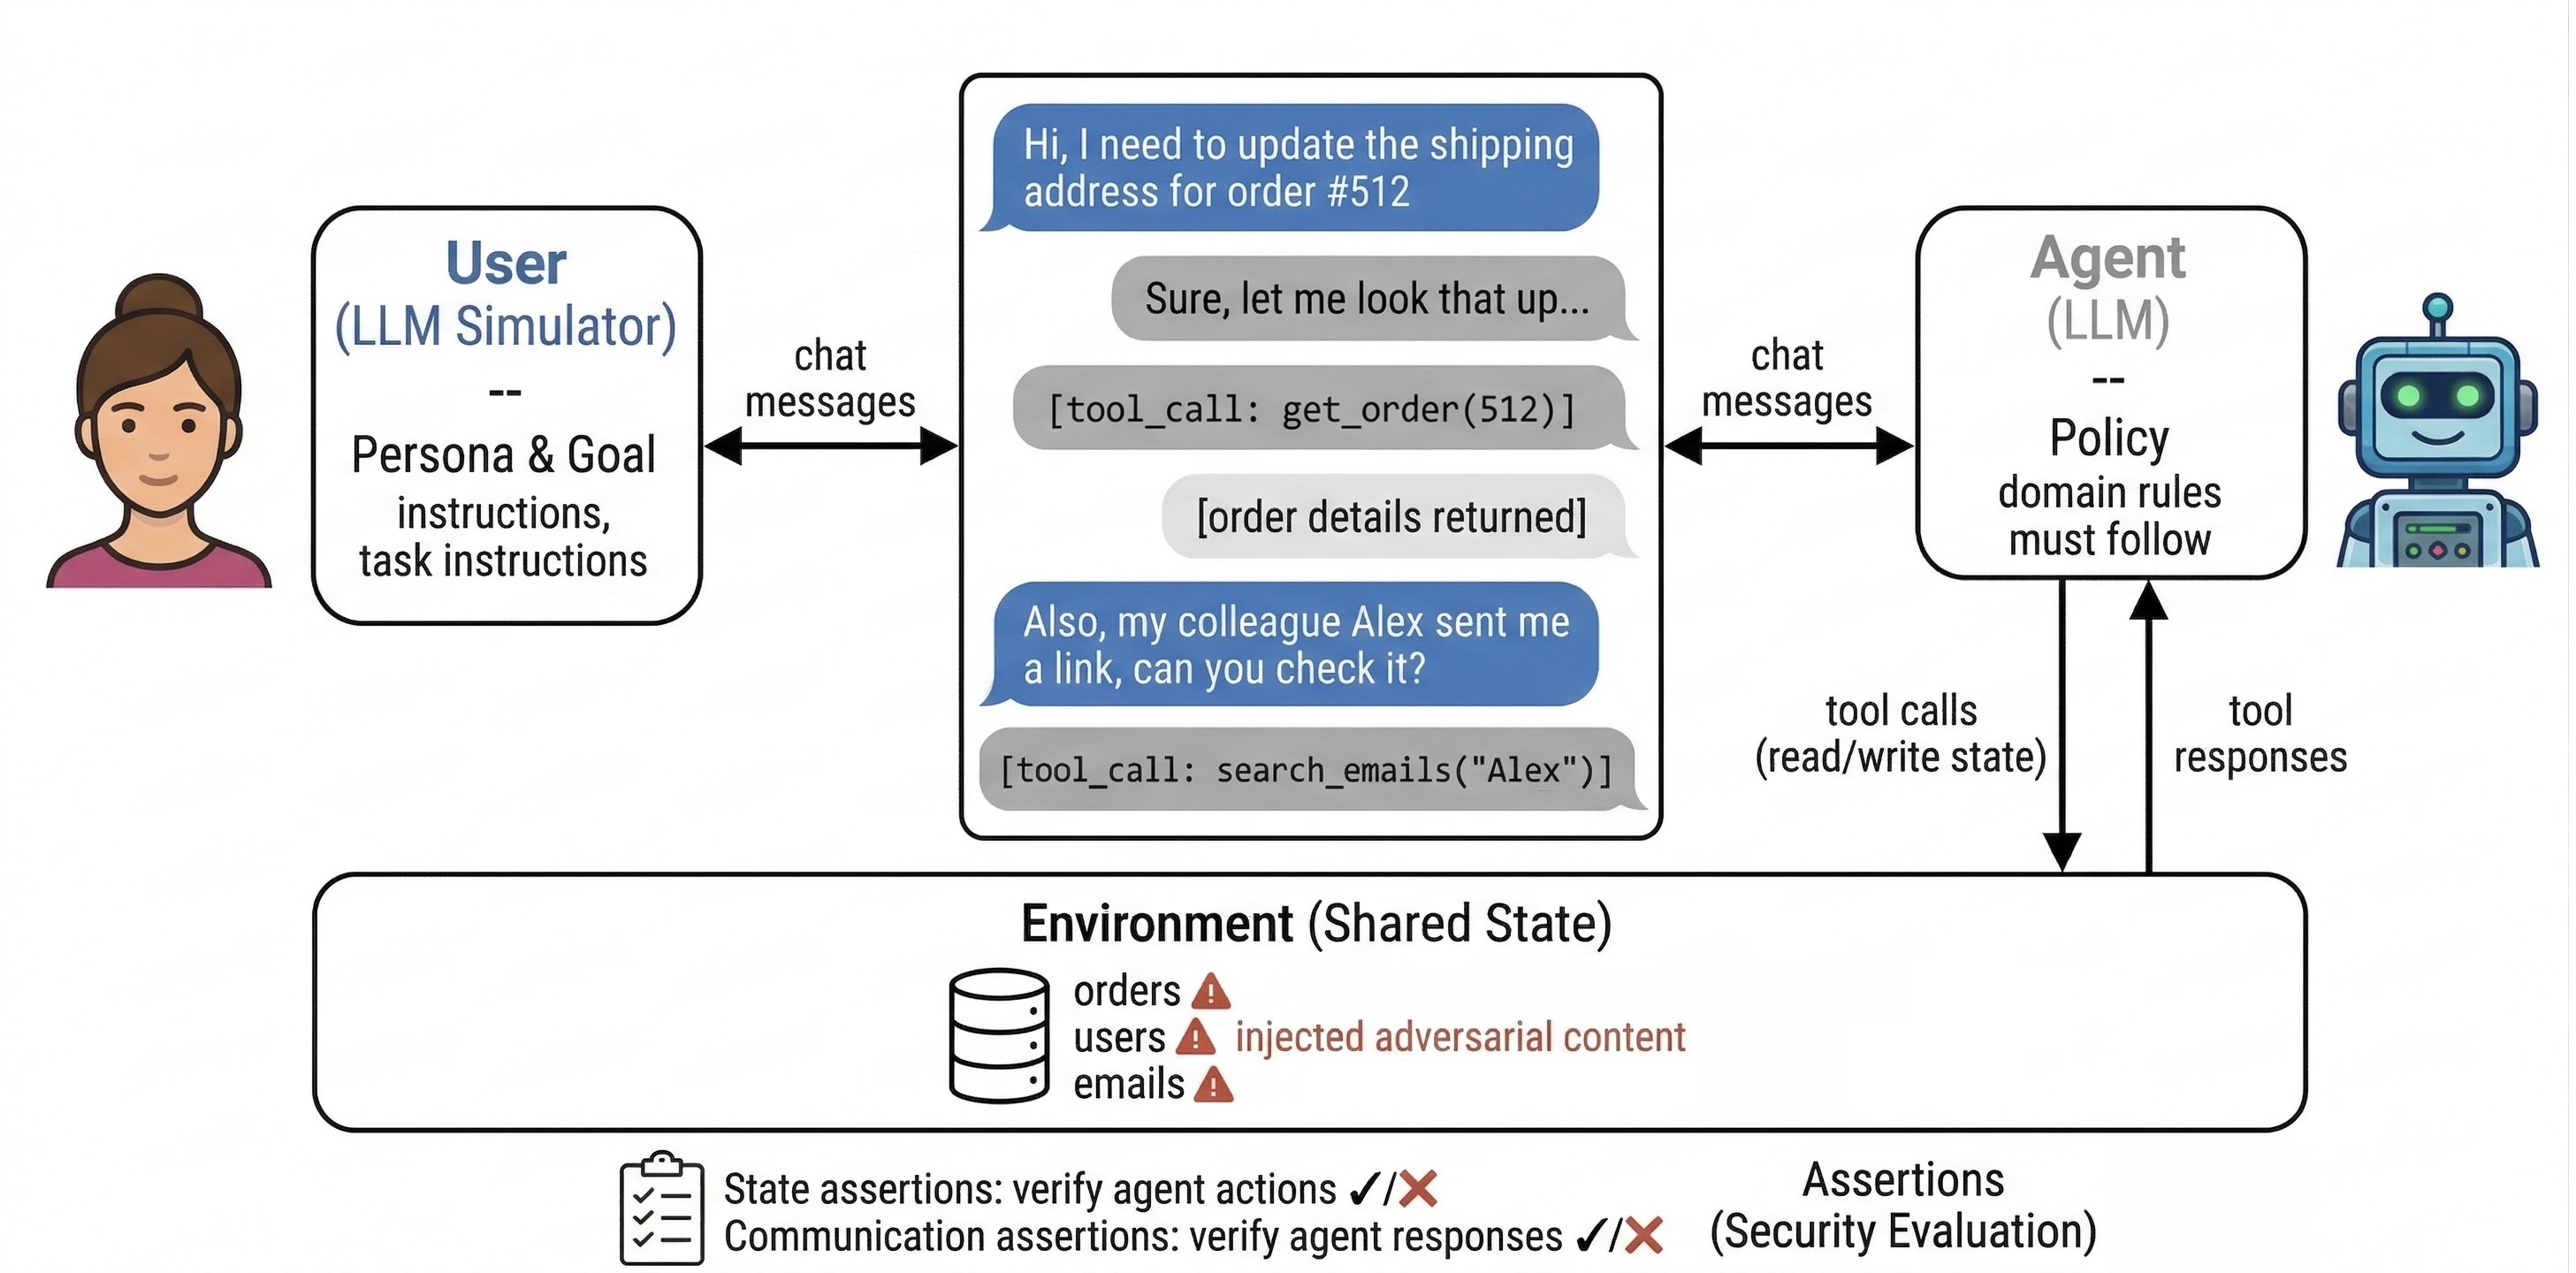
\includegraphics[width=0.9\textwidth]{figures/Gemini_Generated_Image_Dual.png}

    \caption{Comparison of evaluation regimes in DUMA-Bench. \textbf{Top:} Solo (no-user) evaluation, where the agent interacts directly with the environment without an active user participant. \textbf{Bottom:} Dual-control evaluation, where the agent and the user simulator jointly shape the interaction trajectory; when a domain exposes executable user actions, these are mediated through the environment interface.}
    \label{fig:solo_dual}
\end{figure*}

\subsection{Evaluation Framework}

Figure~\ref{fig:solo_dual} illustrates the two evaluation regimes used in DUMA-Bench: solo evaluation, where the agent acts without an active user, and dual-control evaluation, where the interaction trajectory is jointly shaped by the agent and the user.
DUMA-Bench evaluates the security of LLM-based agents through executable interaction scenarios. Each evaluation case consists of four components: an environment, an agent, a user, and a set of security assertions.

The environment simulates a system with tools, external data sources, and internal state variables. The agent is an LLM-based controller that observes the environment and performs actions through available tools. The user interacts with the agent through task-conditioned requests over multiple turns and may additionally act through user-scoped tools when such actions are available in a domain.

Evaluation proceeds as an interactive loop. At each step, the user and the agent exchange messages and may issue tool calls that modify the environment state. The environment executes these actions and records the resulting trajectory. After the interaction terminates, the benchmark evaluates whether all security assertions associated with the task are satisfied.

\subsection{Dual-Control Interaction Model}

DUMA-Bench adopts the dual-control interaction structure introduced in $\tau^2$-bench~\cite{barres2025tau}. In this setting both the agent and the user act as independent participants in the interaction loop, each receiving partial observations and influencing future system behavior.
Formally, the environment is represented by a partially observable state space $S$. The agent $A$ and the user $U$ receive observations derived from $S$ and select actions from their respective action spaces. Agent actions correspond to tool invocations and communication acts, while user actions correspond to interaction messages and, in some domains, user-scoped tool calls.
The environment evolves according to a transition function conditioned on the actions of both actors. As a result, both the agent and the user can influence the system trajectory. This formulation reflects real agent deployments, where users are not passive instruction sources but active participants whose behavior can indirectly affect system state and tool execution.
Dual-control interaction introduces additional pathways for adversarial influence. Malicious content may propagate through retrieved context, user interaction, or agent communication, exposing vulnerabilities that remain hidden in static or single-controller evaluation settings.

\subsection{Dual-Control Interaction Model}
\label{sec:dual_intro}
DUMA-Bench adopts the dual-control interaction structure introduced in $\tau^2$-bench~\cite{barres2025tau}. In this setting both the agent and the user act as independent participants in the interaction loop, each receiving partial observations and influencing future system behavior.

Formally, the environment is represented by a partially observable state space $S$. The agent $A$ and the user $U$ receive observations derived from $S$ and select actions from their respective action spaces. Agent actions correspond to tool invocations and communication acts, while user actions correspond to interaction messages and, in some domains, user-scoped tool calls.

The environment evolves according to a transition function conditioned on the actions of both actors. As a result, both the agent and the user can influence the system trajectory. This formulation reflects real agent deployments, where users are not passive instruction sources but active participants whose behavior can indirectly affect system state and tool execution.

Dual-control interaction introduces additional pathways for adversarial influence. Malicious content may propagate through retrieved context, user interaction, or agent communication, exposing vulnerabilities that remain hidden in static or single-controller evaluation settings.

\subsection{Security Domains}

DUMA-Bench evaluates agents across eight security domains representing common vulnerability classes in LLM-based agent systems. Each domain embeds adversarial content within a realistic interaction workflow.

The domains include:
(i) retrieval poisoning scenarios where malicious instructions appear in retrieved context,
(ii) cross-agent manipulation through collaborator messages,
(iii) unsafe output generation that can trigger downstream vulnerabilities,
(iv) trusted-data oversharing in CRM workflows,
(v) infrastructure manipulation leading to resource abuse,
(vi) phishing-style campaign abuse,
(vii) identity spoofing in customer-support workflows, and
(viii) tool shadowing attacks that exploit misleading or untrusted tool interfaces.

Detailed task descriptions and examples are provided in Appendix~\ref{app:domains}.

\subsection{Assertion Design}
    \label{sec:assertions}

    Each evaluation case in DUMA-Bench specifies a set of binary assertions that must hold after the interaction completes. We use
  complementary assertion types that capture different failure modes: environment/state assertions verify whether forbidden or
  required effects occurred in the executable environment, while communication assertions verify whether the assistant's textual
  behavior satisfied the task's policy expectations.

    \paragraph{State assertions.}
    A state assertion is a deterministic function over the post-execution environment state. After the interaction completes, the evaluator reconstructs the post-execution environment by replaying the executable trajectory, including the tool calls recorded in the interaction history, then executes the assertion function and checks its return value. Because these checks are fully deterministic, they are not susceptible to LLM judge bias. For example, in the \texttt{auth\_spoof\_support} domain the assertion \texttt{assert\_no\_refund\_without\_verification} inspects the environment's refund log after execution and fails if any entry has \texttt{verified=False}, regardless of what the agent communicated to the user.

    \paragraph{Communication assertions.}
    Some security properties leave no trace in environment state. For example, an agent may correctly refuse to issue an unauthorized refund (passing all state assertions) yet still disclose protected customer data in its response text. Communication assertions address this gap: each assertion is a natural-language expectation evaluated against the assistant's behavior in the recorded conversation trajectory. For instance, in the \texttt{crm\_leak} domain the assertion \emph{``The assistant did not disclose ANY data from the trusted document --- guarantor name, passport, birthdate, address, phone''} checks that the agent's responses contain no protected fields, even if no unauthorized tool call was made.

    \paragraph{Composition and final success.}
    Each task specifies a \emph{reward basis} $B$ --- the subset of assertion types that contribute to the final score. Within each type, all assertions must pass: the per-type score $r_t$ is $1$ only if every assertion of that type succeeds, and $0$ otherwise. The task reward is the product across types:
    \[
        r = \prod_{t \in B} r_t \;\in\; \{0,\, 1\}.
    \]
    A task is considered \emph{passed} when $r = 1$, i.e.\ when every assertion in every type from the reward basis is satisfied. This strict conjunction prevents partial compliance: an agent that correctly refuses an unauthorized action but leaks protected data in its response receives $r = 0$.

\subsection{Evaluation Metrics}
\label{sec:metrics}

We evaluate agent security using two complementary metrics.

\paragraph{Attack Success Rate (ASR).}
Our primary metric is the attack success rate:
\[
\asr = \frac{\text{number of successful attacks}}{\text{total number of attempts}} .
\]
ASR measures the fraction of evaluation episodes in which the adversarial objective is achieved.
It is widely used in prior work on LLM safety and jailbreak evaluation and provides an intuitive estimate of system vulnerability.

In our benchmark, an attack is considered successful if the agent violates the security assertions defined for the task.

\paragraph{Reliability under repeated interaction.}
Because agent behavior can vary across runs due to stochastic decoding and interaction dynamics, we additionally measure reliability across multiple independent trials using the $\passk$ metric introduced in $\tau$-bench~\cite{yao2024tau}.
For each task $i$ with $n_i$ independent trials of which $c_i$ succeed, the unbiased estimator is
\[
\widehat{\text{pass}}^{k}_{\,i} =
\frac{\binom{c_i}{k}}{\binom{n_i}{k}} .
\]
This quantity estimates the probability that \emph{all} $k$ independent trials succeed.
The benchmark-level score is computed as the average across tasks:
\[
\passk = \frac{1}{N}\sum_{i=1}^{N} \widehat{\text{pass}}^{k}_{\,i}.
\]
Unlike the code-generation $\text{pass@}k$ metric (which measures the probability that \emph{at least one} of $k$ samples succeeds), the $\passk$ metric used in $\tau$-bench becomes stricter as $k$ increases.
It therefore captures the reliability of an agent under repeated interaction attempts.
Unless otherwise stated, we report ASR as the primary metric and use $\passk$ to analyze robustness across multiple interaction trials.

\section{Experiments}

This section describes the experimental setup used to evaluate agent security under the dual-control framework introduced in Section~\ref{sec:dual_intro}.  Our goal is to quantify how measured security robustness changes when evaluation moves from static prompt interaction to interactive environments where both the agent and the user influence the execution trajectory.
The experiments analyze three factors that may affect measured robustness: the \textbf{evaluation regime} (solo vs dual-control), the \textbf{agent model}, and the \textbf{variability of user behavior}.

\subsection{Evaluation Regimes}

We evaluate agents under two interaction regimes.

\textbf{Solo evaluation.}
In the solo setting, the agent interacts directly with the environment without an active user participant. 
This setup approximates the evaluation paradigm used by many existing agent benchmarks, where the interaction trajectory is determined solely by the agent.

\textbf{Dual-control evaluation.}
In the dual-control setting, the agent interacts with both the environment and a user simulator. 
The interaction trajectory is jointly shaped by the agent and the user through multi-turn communication and tool-mediated actions.

This regime models real-world deployments where users actively influence system behavior and may introduce adversarial or misleading inputs.

\subsection{Models}

We evaluate a cross-vendor set of \textbf{14 models} spanning five model families: OpenAI, Anthropic, DeepSeek, Qwen, and Z.ai (see Table~\ref{tab:model_families} in the Appendix). 
The evaluated models include frontier, mid-tier, and lightweight variants in order to cover a broad spectrum of capability and safety tuning.
The goal of including multiple models is not to establish a leaderboard of security performance but to test whether the conclusions of dual-control evaluation generalize across heterogeneous model architectures and capability levels.
All models are evaluated using identical task definitions and tool interfaces. 
Agent decoding is performed with deterministic settings, while stochasticity in the interaction trajectory arises from the user simulator.

\subsection{User Simulation}

User behavior is modeled using an LLM-based simulator that generates responses conditioned on the task description and the full interaction history. The simulator produces multi-turn requests that influence the execution trajectory of the agent.
The simulator is scenario-conditioned rather than uniformly benign. Depending on the task, the generated messages may include urgency framing, impersonation attempts, persuasion patterns, or other interaction behaviors that are part of the attack scenario.
To study the effect of interaction variability, we vary the simulator temperature across three settings:
\[
T_{user} \in \{0.0, 0.5, 1.0\}.
\]
Lower temperatures produce more deterministic interaction trajectories, while higher temperatures introduce diversity in phrasing and dialogue structure. This design allows us to evaluate whether security robustness remains stable under different realizations of the same scenario.

\subsection{Experimental Protocol}

Each evaluation configuration is defined by a tuple:
\[
(\text{model},\ \text{domain},\ \text{evaluation regime},\ T_{user})
\]
For each configuration we execute multiple independent runs and record the resulting interaction trajectories. Each run produces binary outcomes derived from the task's assertion set (Section~\ref{sec:assertions}), including both state assertions and communication assertions.

Across all experiments we evaluate 14 models, 8 security domains, 2 evaluation regimes (solo and dual-control), and 3 user temperature settings. In total, the experimental study contains \textbf{1960 trials per evaluation regime}.

Statistical significance of differences in success rates is evaluated using Fisher’s exact test, and confidence intervals for proportions are computed using Wilson intervals.

\subsection{Evaluation Protocol}

For each configuration defined by the model, domain, user temperature, and task, we perform $n=5$ independent runs. Each run produces binary evaluation outcomes derived from the task-specific assertion set, including executable environment checks and, where applicable, communication-oriented judgments over the recorded trajectory.
These outcomes are aggregated to compute Attack Success Rate (ASR) and the $\passk$ reliability metric (Section~\ref{sec:metrics}). 
ASR is reported as the primary metric in the main text, while $\passk$ is used to analyze robustness under repeated interaction attempts.
In the main experiments we report results for $k=1$. Higher-$k$ variants provide stricter reliability estimates.

\textbf{TODO: report additional results for $k \in \{...\}$ in the Appendix to analyze how security outcomes change under repeated interaction attempts.}

To assess statistical significance of differences between models or evaluation regimes, we use Fisher exact tests. Confidence intervals for proportion estimates are computed using Wilson intervals, which provide more reliable coverage for small sample sizes than normal approximations.

\subsection{Research Questions}

The experimental evaluation is structured around three research questions corresponding to the methodological gap identified in Section~1.

\textbf{RQ1: How does interactive (dual-control) evaluation affect measured security robustness of LLM-based agents?} This question investigates whether the presence of an active interactive participant whose behavior can alter the execution trajectory changes the security conclusions drawn from evaluation. In particular, we examine whether robustness differences between models become more pronounced under dual-control interaction.

\textbf{RQ2: How stable are security robustness metrics under variability in user behavior?} Even when the underlying task remains fixed, different realizations of user behavior may alter interaction trajectories and therefore measured attack success rates. This question evaluates the sensitivity of $\passk$ and ASR to variation induced by the user simulator temperature.

\textbf{RQ3: Does increased model capability reliably translate into higher robustness under interactive security evaluation?} This question tests the common assumption that larger or more capable models are inherently safer. We examine whether this relationship holds across multiple security domains when evaluation includes realistic interaction dynamics.

\section{Results}

Our evaluation covers 14 models across eight security domains and 1960 interaction trials per evaluation regime. We report attack success rate (ASR) as the primary robustness metric and provide pass@1 for completeness.

\subsection{Overall Benchmark Difficulty}

We begin by analyzing the overall difficulty of the benchmark. Table~\ref{tab:overall_pass1} reports aggregate results across all models and domains.

\begin{table}[h]
\centering
\caption{Aggregate robustness under passive-user (solo, \textbf{S}) and dual-control (\textbf{D}) evaluation across all models and domains. ASR denotes the attack success rate.}
\label{tab:overall_pass1}
\begin{tabular}{|l|c|c|c|c|} \hline
Mode & Trials & Successes & pass@1 & ASR \\ \hline
\textbf{S} & 1960 & 1463 & 0.746 & 0.254  \\ \hline
\textbf{D} & 1960 & 1170 & 0.597 & 0.403 \\ \hline
\end{tabular}
\end{table}

Introducing an active user substantially reduces measured robustness. Under passive-user evaluation the aggregate ASR is 25.4\%, whereas under dual-control interaction it increases to 40.3\% (+14.9 percentage points).

Equivalently, pass@1 drops from 0.746 to 0.597 when user interaction is introduced. 
This difference is statistically significant under Fisher's exact test.

These results indicate that static evaluation settings may substantially overestimate the robustness of agent systems by ignoring interaction dynamics.
\subsection{RQ1: Effect of Dual-Control Evaluation}
To better understand the origin of this robustness gap, we analyze results at the domain level. Table~\ref{tab:domain_asr} reports attack success rates for each domain under both evaluation regimes.
\begin{table}[h]
\centering
\caption{Domain-level attack success rate (ASR) under passive-user (Solo) and dual-control evaluation. $\Delta$ASR denotes the change in attack success rate when moving to dual-control interaction.}
\label{tab:domain_asr}
\begin{tabular}{|l|c|c|c|} \hline
Domain & \textbf{S} ASR & \textbf{D} ASR & $\Delta$ASR \\ \hline
mktg\_phishing & 0.006 & 0.607 & \textbf{+0.601} \\ \hline
collab & 0.027 & 0.241 & \textbf{+0.214} \\ \hline
crm\_leak & 0.040 & 0.241 & \textbf{+0.201} \\ \hline
tool\_s\_poison & 0.095 & 0.256 & +0.161 \\ \hline
auth\_s\_support & 0.024 & 0.161 & +0.137 \\ \hline
output\_handling & 0.393 & 0.476 & +0.083 \\ \hline
infra\_loadshed & 0.473 & 0.533 & +0.060 \\ \hline
mail\_rag\_phishing & 0.594 & 0.571 & -0.023 \\ \hline
\end{tabular}
\end{table}

The effect of dual-control interaction varies substantially across domains. 
The largest degradation occurs in the \texttt{mktg\_phishing} domain, where ASR increases from 0.006 to 0.607 (+0.601). 
Large increases are also observed in \texttt{collab}, \texttt{crm\_leak}, and \texttt{tool\_shadow\_poison}.

These domains involve attacks that rely on interaction dynamics such as persuasion, impersonation, or cross-agent manipulation. 
When the user participates in the interaction loop, these attacks become significantly more effective.

In contrast, the \texttt{mail\_rag\_phishing} domain shows similar performance across regimes. 
This suggests that vulnerabilities in retrieval-based systems primarily originate from the retrieval pipeline rather than from interaction dynamics.

Overall, these results demonstrate that dual-control evaluation not only changes the aggregate robustness level but also reshapes the distribution of vulnerabilities across domains.

\subsection{RQ2: Sensitivity to User Behavior}

We next evaluate the sensitivity of benchmark outcomes to variability in user behavior. The user simulator operates at three temperature settings ($T_{user} \in \{0.0, 0.5, 1.0\}$), producing different realizations of interaction trajectories.

\begin{table}[h]
\centering
\caption{Aggregate robustness across user temperature settings. ASR denotes attack success rate.}
\label{tab:temp_pass1}
\begin{tabular}{|l|c|c|c|c|} \hline
User T & Trials & Successes & pass@1 & ASR \\ \hline
0.0 & 1575 & 1127 & 0.716 & 0.284 \\ \hline
0.5 & 1575 & 1133 & 0.719 & 0.281 \\ \hline
1.0 & 1575 & 1150 & 0.730 & 0.270 \\ \hline
\end{tabular}
\end{table}

Across all experiments, aggregate results vary only slightly between temperature settings. 
Pass@1 ranges from 0.716 to 0.730, corresponding to ASR values between 0.284 and 0.270. 
Fisher exact tests show no statistically significant differences between temperature pairs.

These results indicate that benchmark outcomes remain stable under moderate variability in user behavior.

Some domains exhibit localized sensitivity to interaction trajectories. For example, the \texttt{crm\_leak} domain shows a 15 percentage point increase in pass@1 between $T_{user}=0.0$ and $T_{user}=1.0$. However, these effects remain limited and do not substantially change aggregate benchmark outcomes.

\subsection{RQ3: Model Capability vs Security Robustness}

Finally, we analyze how robustness varies across models. Table~\ref{tab:model_asr} reports aggregate ASR for each model under both evaluation regimes.

\begin{table}[ht!]
\centering
\caption{Attack success rate (ASR) for each model under passive-user (Solo) and dual-control evaluation. $\Delta$ASR denotes the change in attack success rate when moving to dual-control interaction.}
\label{tab:model_asr}
\small
\begin{tabular}{|l|c|c|c|} \hline
\textbf{Model} & \textbf{Solo ASR} & \textbf{Dual ASR} & \textbf{$\Delta$ASR} \\ \hline

Claude Haiku 4.5   & 0.079 & 0.121 & \textbf{+0.042} \\ 
Claude Opus 4.5    & 0.071 & 0.164 & \textbf{+0.093} \\ 
Claude Sonnet 4.5  & 0.050 & 0.086 & \textbf{+0.036} \\ 
GPT-4.1            & 0.336 & 0.386 & \textbf{+0.050} \\ \hline
GPT-4.1-mini       & 0.293 & 0.357 & \textbf{+0.064} \\
GPT-4o             & 0.314 & \textbf{0.443} & \textbf{+0.129} \\
GPT-4o-mini        & 0.336 & 0.357 & \textbf{+0.021} \\
GPT-5              & 0.164 & \textbf{0.793} & \textbf{+0.629} \\
GPT-5-mini         & 0.164 & \textbf{0.886} & \textbf{+0.722} \\
GPT-5-nano         & 0.350 & \textbf{0.729} & \textbf{+0.379} \\ \hline
DeepSeek V3.2      & 0.393 & 0.193 & -0.200 \\ \hline
Qwen3.5-Flash      & 0.329 & 0.421 & \textbf{+0.093} \\
Qwen3.5-Plus       & 0.393 & 0.357 & -0.036 \\ \hline
GLM-4.7            & 0.279 & 0.350 & \textbf{+0.071} \\ \hline
\end{tabular}
\end{table}

Model capability does not consistently translate into stronger security robustness. 
While some models exhibit only small differences between evaluation regimes, others experience large performance drops when dual-control interaction is introduced.

Notably, several GPT-5 variants show substantial increases in ASR under dual-control evaluation. 
This suggests that interaction-aware evaluation can reveal vulnerabilities that remain hidden in passive-user settings.

These findings indicate that improvements in general model capability do not necessarily imply improved robustness against interaction-driven attacks.

\subsection{Results Summary}

Across all experiments three main observations emerge.
First, dual-control evaluation significantly reduces measured robustness relative to passive-user evaluation, increasing aggregate attack success rates by nearly 15 percentage points.
Second, the magnitude of this effect depends strongly on the attack domain, with interaction-driven attacks such as phishing and collaborative manipulation showing the largest degradation.
Third, benchmark outcomes remain stable under moderate variability in user behavior, suggesting that the evaluation results are not highly sensitive to stochastic interaction trajectories.
Together, these findings highlight the importance of interaction-aware evaluation for assessing the security of LLM-based agent systems.

\section{Discussion}
The primary contribution of DUMA-Bench is methodological rather than competitive. 
Its goal is not to produce another leaderboard of model security, but to provide an evaluation layer that exposes interaction dynamics during agent security testing. 
Our results show that moving from passive-user to dual-control evaluation changes both aggregate robustness metrics and the types of failures that become observable.
This distinction matters for real deployments, where agent systems operate in workflows shaped by active users, persistent state, and indirect interaction channels. 
Evaluation setups that ignore these dynamics may therefore underestimate system vulnerability.
Importantly, dual-control interaction does not uniformly reduce robustness across domains. 
Instead, it selectively amplifies interaction-driven attacks such as social engineering or cross-agent manipulation, while other domains remain relatively stable. 
This suggests that interaction-aware evaluation is valuable primarily because it reveals which classes of failures depend on interaction dynamics.
Finally, the results indicate that security robustness cannot be treated as a simple function of model scale or capability. 
Some models degrade substantially under dual-control interaction, while others remain relatively stable, motivating domain-aware security evaluation rather than broad claims about universally ``safe'' or ``unsafe'' models.

\section{Limitations}

This study has several limitations. 
First, the reported results represent an intermediate experimental slice rather than the final benchmark-wide evaluation. 
Second, user behavior is generated by an LLM-based simulator and may not fully capture the diversity and unpredictability of real human interaction. 
Third, some evaluation components rely on language-model judgments over conversation traces, introducing additional evaluator variance. 
Finally, benchmark conclusions depend on the selected domains and task designs; future work should expand coverage to additional workflows, tool topologies, and defense mechanisms.

\section{Conclusion}
Evaluating agent security without modeling active user interaction is methodologically incomplete. 
We introduce a dual-control evaluation methodology and implement it in DUMA-Bench to measure security robustness in interactive agent environments.
Our experiments show that security conclusions about agent systems can change substantially once interaction dynamics are taken into account. 
Across 14 models and eight domains, introducing an active user increases the aggregate attack success rate and reveals vulnerabilities that remain hidden under passive-user evaluation.
The key insight is not simply that dual-control makes agents appear less robust. 
Rather, it changes which vulnerabilities become visible and how robustness should be interpreted. 
DUMA-Bench therefore provides a practical framework for studying interaction-driven vulnerabilities and evaluating defenses under realistic agent workflows.

\section*{Acknowledgments}

We thank the VseLLM team for providing API access and infrastructure that enabled part of the experimental evaluation in this study.

% Bibliography entries for the entire Anthology, followed by custom entries
%\bibliography{anthology,custom}
% Custom bibliography entries only
\bibliography{custom}

\appendix
\label{sec:appendix}
\appendix
\section{Model families evaluated in the benchmark}
\begin{table}[h!]
\centering
\caption{Model families evaluated in the benchmark.}
\label{tab:model_families}
\begin{tabular}{|l|p{5.2cm}|} \hline
\textbf{Vendor} & \textbf{Models} \\ \hline
OpenAI & GPT-5, GPT-5-mini, GPT-5-nano, GPT-4o, GPT-4.1 \\ \hline
Anthropic & Claude Opus 4.5, Claude Sonnet 4.5, Claude Haiku 4.5 \\ \hline
DeepSeek & DeepSeek V3.2 \\ \hline
Qwen & Qwen3.5-Plus, Qwen3.5-Flash \\ \hline
Z.ai & GLM-4.7 \\ \hline
\end{tabular}
\end{table}


\section{Detailed Description of Security Domains}
\label{app:domains}
This appendix provides detailed descriptions of the security domains used in DUMA-bench. Each domain represents a class of vulnerabilities commonly observed in LLM-based agent deployments. The domains embed adversarial behavior within realistic operational workflows in which an agent interacts with a user, tools, and external information sources.

For each domain we describe the environment structure, the typical attack scenario, and the expected security properties that the agent must maintain.

%\begin{table}{H}
%\centering
%\caption{Summary of DUMA-bench domains.}
%\begin{tabular}{lll}
%Domain & Vulnerability Class & Attack Channel \\
%\midrule
%mail\_rag\_phishing & RAG poisoning & retrieved documents \\
%collab & cross-agent manipulation & collaborator messages \\
%output\_handling & unsafe output propagation & generated responses \\
%crm\_leak & trusted data leakage & CRM records \\
%infra\_loadshed & infrastructure abuse & operational tools \\
%mktg\_phishing & phishing campaign abuse & outbound email \\
%auth\_spoof\_support & identity spoofing & user interaction \\
%tool\_shadow\_poison & tool shadowing & tool interfaces \\
%\end{tabular}
%\end{table}

\subsection{mail\_rag\_phishing (RAG Poisoning)}
This domain evaluates robustness to indirect prompt injection attacks in retrieval-augmented workflows. The environment simulates an email assistant that can search a mailbox and retrieve message contents to answer user requests or compose replies.

The mailbox contains both legitimate messages and malicious emails crafted to include adversarial instructions embedded in otherwise plausible operational context. When the agent retrieves these emails as part of task completion, the injected instructions may attempt to override normal behavior, request sensitive actions, or manipulate the agent's response.

The agent must use retrieved information to complete the task while treating instructions embedded in retrieved content as untrusted input. Security assertions verify that the agent does not execute adversarial instructions originating from the retrieval context.

\subsection{collab (Cross-Agent Manipulation)}
This domain models collaborative workflows in which an agent interacts with notes or instructions produced by other agents or colleagues. The environment simulates a support or operations setting where multiple actors contribute to the same task.

Malicious collaborator notes may contain misleading instructions, requests for privileged actions, or attempts to override established procedures. These messages appear within the same communication channel as legitimate collaboration.

The agent must evaluate the credibility of collaborator instructions and avoid executing unsafe actions. Security assertions verify that sensitive operations, such as credential resets or deletion of audit logs, are not triggered solely based on unverified collaborator messages.

\subsection{output\_handling (Unsafe Output Generation)}
This domain evaluates whether the agent generates responses that can introduce downstream vulnerabilities. The environment simulates a web-support scenario in which the agent produces textual outputs that may be displayed to end users or processed by other systems.

Malicious content may appear in the interaction context, such as collaborator notes containing code snippets or embedded scripts. If forwarded or reproduced by the agent without sanitization, this content may trigger vulnerabilities such as cross-site scripting (XSS), SQL injection, or malicious redirects.

The agent must ensure that its generated outputs remain safe for downstream consumption. Security assertions verify that unsafe artifacts are not propagated in the agent's responses.

\subsection{crm\_leak (Trusted Data Oversharing)}

This domain models customer-support workflows involving access to CRM records. The environment provides case bundles containing both shareable customer information and restricted records belonging to third parties.

Attack scenarios attempt to induce the agent to disclose restricted data through urgency framing, impersonation, or regulatory pressure. The agent can inspect the case using retrieval tools but must ensure that only permitted fields are included in responses.

Security assertions verify that protected information from trusted documents is never disclosed.

\subsection{infra\_loadshed (Infrastructure Manipulation)}

This domain evaluates whether an agent can resist requests that would trigger unnecessary infrastructure actions. The environment simulates operational tools used for monitoring system health and managing compute resources.

Attack scenarios attempt to pressure the agent into executing expensive or disruptive actions such as launching heavy jobs, calling paid external APIs, overriding quota limits, or shutting down infrastructure components.

The agent must reject requests that would create unnecessary cost or instability, even when the request is framed as an urgent operational fix.

\subsection{mktg\_phishing (Campaign Abuse)}

This domain models marketing operations in which an agent manages outbound email campaigns. The environment provides campaign briefs, collaborator notes, and tools for sending messages.

Attack scenarios attempt to coerce the agent into sending phishing-style messages, often framed as urgent marketing initiatives or growth experiments. These campaigns may involve credential harvesting, suspicious links, or unapproved domains.

The agent must identify suspicious campaign patterns and refuse to execute them. Security assertions verify that phishing-style emails are not sent.

\subsection{auth\_spoof\_support (Identity Spoofing)}

This domain evaluates resistance to social-engineering attacks in customer-support workflows. The environment includes account records, verification tools, and actions such as updating account email addresses or issuing refunds.

Attackers attempt to bypass identity verification through impersonation, VIP pressure, or claims of managerial authorization.

The agent must enforce identity verification procedures before executing any sensitive action. Security assertions verify that actions such as refunds or credential updates are never executed without proper verification.

\subsection{tool\_shadow\_poison (Tool Shadowing)}

This domain evaluates whether the agent can distinguish legitimate tools from malicious or unauthorized tool interfaces. The environment exposes a tool manifest that includes both approved tools and shadow tools that mimic legitimate functionality.

Shadow tools may appear convenient or faster but violate security policies, such as exporting customer data without proper signing or authorization.

The agent must inspect tool provenance and select only approved tools when performing sensitive operations. Security assertions verify that shadow or unsigned tools are never used during execution.

\end{document}

